
\documentclass{beamer}
\usepackage{multicol}
\usepackage{braket}
\usepackage{tikzit}
\input{zx-calculus.tikzstyles}
\usepackage{tikz}


\usetheme{metropolis}           % Use metropolis theme
\title{Reconfiguring staggered quantum walks with ZX}
\date{November 5, 2024}
\author{Bruno Jardim \and Jaime Santos \and Luís Soares Barbosa}
\institute{HASLab - INESCTEC}
\begin{document}
\maketitle

\section{Introduction}
\begin{frame}{Introduction}

\begin{itemize}
\item Optimization of quantum circuits can be seen as a \emph{reconfiguration} process. 
\item Indeed the interpretation of such circuits as ZX-diagrams provides a flexible description of quantum computations graphically.
\end{itemize}

\begin{block}{Objective}
Resort to the ZX-calculus to optimize a specific quantum walk.
\end{block}
\end{frame}


\section{Staggered Quantum Walks}
\begin{frame}{Staggered Quantum Walks}
	Thought of as the quantum counterpart to classical random walks, quantum walks provide an interesting technique in algorithmic design, with  applications in unstructured search, graph algorithmics and communication protocols.
	
	\begin{block}{Staggered Quantum Walks}
	\begin{itemize}
	\item The Staggered Quantum Walks is a recent and very general variant of discrete quantum walks 
	\item It avoids the use of a coin to direct the walker evolution, exploring the underlying graph structure to build an evolution operator based on local unitaries induced by adjacent vertices.
	\end{itemize}
\end{block}
	
\end{frame}


\section{Introduction to the ZX-Calculus}
\begin{frame}{ZX-Calculus}
	The ZX-calculus is diagrammatic language for reasoning about linear maps between qubits and, as such, about quantum computation in general.


\end{frame}

\begin{frame}{ZX-Calculus - Generators}
	\tikzfig{zx-spiders}
\end{frame}
\begin{frame}{ZX-Calculus - Rewrite Rules}



	\begin{multicols}{2}
		\begin{itemize}
			\item Spider Fusion
			      \resizebox{0.4\textwidth}{!}{% 
				      \tikzfig{rule-sf}
			      }%
			\item Identity Removal
			      \resizebox{0.4\textwidth}{!}{% 
				      \tikzfig{rule-id}
			      }%
			\item Color Change
			      \resizebox{0.4\textwidth}{!}{% 
				      \tikzfig{rule-colour-change}
			      }%
			\item Hadamard Identity
			      \resizebox{0.4\textwidth}{!}{% 
				      \tikzfig{rule-had-id}
			      }%
			\item Bialgebra
			      \resizebox{0.4\textwidth}{!}{% 
				      \tikzfig{rule-bialg}
			      }%
			\item $\pi$-commutation
			      \resizebox{0.4\textwidth}{!}{% 
				      \tikzfig{rule-pi-com}
			      }%
			\item Hopf
			      \resizebox{0.4\textwidth}{!}{% 
				      \tikzfig{rule-hopf}
			      }%
			\item State copy
			      \resizebox{0.4\textwidth}{!}{% 
				      \tikzfig{rule-state-copy}
			      }%


		\end{itemize}
	\end{multicols}



\end{frame}
\section{Optimizing Staggerd Quantum Walks with ZX}

\begin{frame}{Staggerd Quantum Walk - Circuit}
	A general implementation of a Staggered Quantum Walk for a line graph.

	\ctikzfig{sqw-circuit}

\end{frame}


\begin{frame}{Staggerd Quantum Walk - ZX-diagram}
	A concrete implementation of a Staggered Quantum Walk for a line graph with 3 qubits and the state $\ket{4}$ as the initial state.

	\ctikzfig{1-step-sqw}

\end{frame}
\begin{frame}{Staggerd Quantum Walk - ZX-diagram}
	The previous diagram utilizes a notation from the ZH-calculus for the Tofolli gates that greatly simplifies the diagram. Expanding the Tofolli gates it yields
	\begin{align*}
		\resizebox{0.9\textwidth}{!}{% 
			\tikzfig{1-step-expanded}
		}%
	\end{align*}
\end{frame}
\begin{frame}{Staggerd Quantum Walk - ZX-diagram}
	\begin{align*}
		\resizebox{0.9\textwidth}{!}{% 
			\tikzfig{1-step-trivial}
		}%
	\end{align*}
\end{frame}

\begin{frame}{Staggerd Quantum Walk - ZX-diagram}
	Unfortunately this is the limit one can reasonably optimize the circuit by hand.
	
	This is where PyZX comes in.
\end{frame}

\section{PyZX}
\begin{frame}{Automated Diagrammatic Rewriting - PyZX}
	PyZX is a Python tool implementing the theory of ZX-calculus. 
	
	\begin{block}{Capabilities}
		\begin{itemize}
			\item Creation
			\item Visualization
			\item Automated rewriting of large-scale quantum circuits
		\end{itemize}
	\end{block}
\end{frame}

\begin{frame}{Automated Diagrammatic Rewriting - PyZX}
	\begin{itemize}
		\item The \texttt{full\_reduce} method implemented in PyZX may reduce the circuit T-count in about $50\%$
	\end{itemize}
	
	\begin{block}{Consequece}
		The resulting diagram no longer resembles a circuit, making direct comparisons with the original one difficult.
	\end{block}
\end{frame}

\begin{frame}{Staggered Quantum Walk - Graph-like}
	
	\begin{align*}
		\resizebox{0.9\textwidth}{!}{% 
			\tikzfig{graph-like}
		}%
	\end{align*}
\end{frame}

\begin{frame}{Optimization Comparison - Total Number of Gates}
	
	\begin{table}[H]
		
		\centering
		\resizebox{\textwidth}{!}{\begin{tabular}{|l|cccc|}
			
		\hline
									   & \multicolumn{4}{l|}{Number of steps in the staggered quantum walk:}                                   \\ \hline
		Optimizations used:          & \multicolumn{1}{c|}{1}  & \multicolumn{1}{c|}{2}  & \multicolumn{1}{c|}{4}   & 8   \\ \hline
		None            & \multicolumn{1}{c|}{39} & \multicolumn{1}{c|}{77} & \multicolumn{1}{c|}{153} & 305 \\ \hline
		Simple     & \multicolumn{1}{c|}{31} & \multicolumn{1}{c|}{59} & \multicolumn{1}{c|}{115} & 227 \\ \hline
		Full-reduce + fusion/id/to\_rg & \multicolumn{1}{c|}{37} & \multicolumn{1}{c|}{47} & \multicolumn{1}{c|}{72}  & 118 \\ \hline
	
		\end{tabular}
		}
		%\label{tab:total-gates}
		\end{table}
		
\end{frame}	
\begin{frame}{Optimization Comparison - T-count}	
	\begin{table}[H]
		\centering
		\resizebox{\textwidth}{!}{\begin{tabular}{|l|cccc|}
		\hline
									   & \multicolumn{4}{l|}{Number of steps in the staggered quantum walk:}                                  \\ \hline
		Optimizations used:          & \multicolumn{1}{c|}{1}  & \multicolumn{1}{c|}{2}  & \multicolumn{1}{c|}{4}  & 8   \\ \hline
		None            & \multicolumn{1}{c|}{16} & \multicolumn{1}{c|}{32} & \multicolumn{1}{c|}{64} & 128 \\ \hline
		Simple       & \multicolumn{1}{c|}{16} & \multicolumn{1}{c|}{32} & \multicolumn{1}{c|}{64} & 128 \\ \hline
		Full-reduce + fusion/id/to\_rg & \multicolumn{1}{c|}{10} & \multicolumn{1}{c|}{16} & \multicolumn{1}{c|}{28} & 52  \\ \hline
		\end{tabular}}
		\end{table}
		
\end{frame}

\section{An alternative evolution operator}
\begin{frame}{An alternative evolution operator}	
When analyzing the  ZX diagram for a long staggered quantum walk (i.e. with more than 5 steps)  a pattern starts to emerge, repeating itself as many times as  the number of steps considered.
\end{frame}

\begin{frame}{An alternative evolution operator}	
	\begin{align*}
		\tikzfig{sqw-pattern-standard}
	\end{align*}
	where $\alpha_n = \pm \frac{\pi}{4}$ and $\beta_n = \frac{2\pi}{3} + m\pi$, with $m=0$ or $m=1$.
\end{frame}

\begin{frame}{An alternative evolution operator - Generalization}	
	\begin{align*}
		\resizebox{0.9\textwidth}{!}{
		\tikzfig{sqw-pattern-generalization}
		}
	\end{align*}
\end{frame}
\begin{frame}{An alternative evolution operator - Rationale}	
	\begin{itemize}
		\item Creates a uniform distribution over a certain number of states.
		\item Applies a rotation that makes some states more likely than others.
		\item Spreads these probabilities over the remaining states using CNOT gates.
	\end{itemize}

	This also explains why the pattern only shows up in staggered quantum walks over a certain length. 
\end{frame}
\begin{frame}{An alternative evolution operator - Advantages}	
	\begin{itemize}
		\item Reduces the total amount of gates needed to represent the evolution of the quantum walk
		\item Only uses gates controlled by at most 1 qubit
		\item To go from an $n$-qubit to an $n+1$ qubit quantum walk, all that needs to be done is to add two more XCX-gates
	\end{itemize}
\end{frame}
\begin{frame}{An alternative evolution operator - Advantages}	
	In general, this makes the alternative operator much more efficient with respect to the total number of gates used, leading to lower depth  and, therefore, potentially less error-prone circuits.
\end{frame}

\begin{frame}{An alternative evolution operator - Disadvantages}	
However, a number of challenges remain, requiring further investigation. 
	\begin{itemize}
		\item Most suitable choice of parameters for $\alpha_n$ and $\beta_n$.
		\item Whether and how they depend on the number of qubits used in a particular staggered walk
	\end{itemize}
\end{frame}
\begin{frame}{An alternative evolution operator - Example}	
	\begin{align*}
		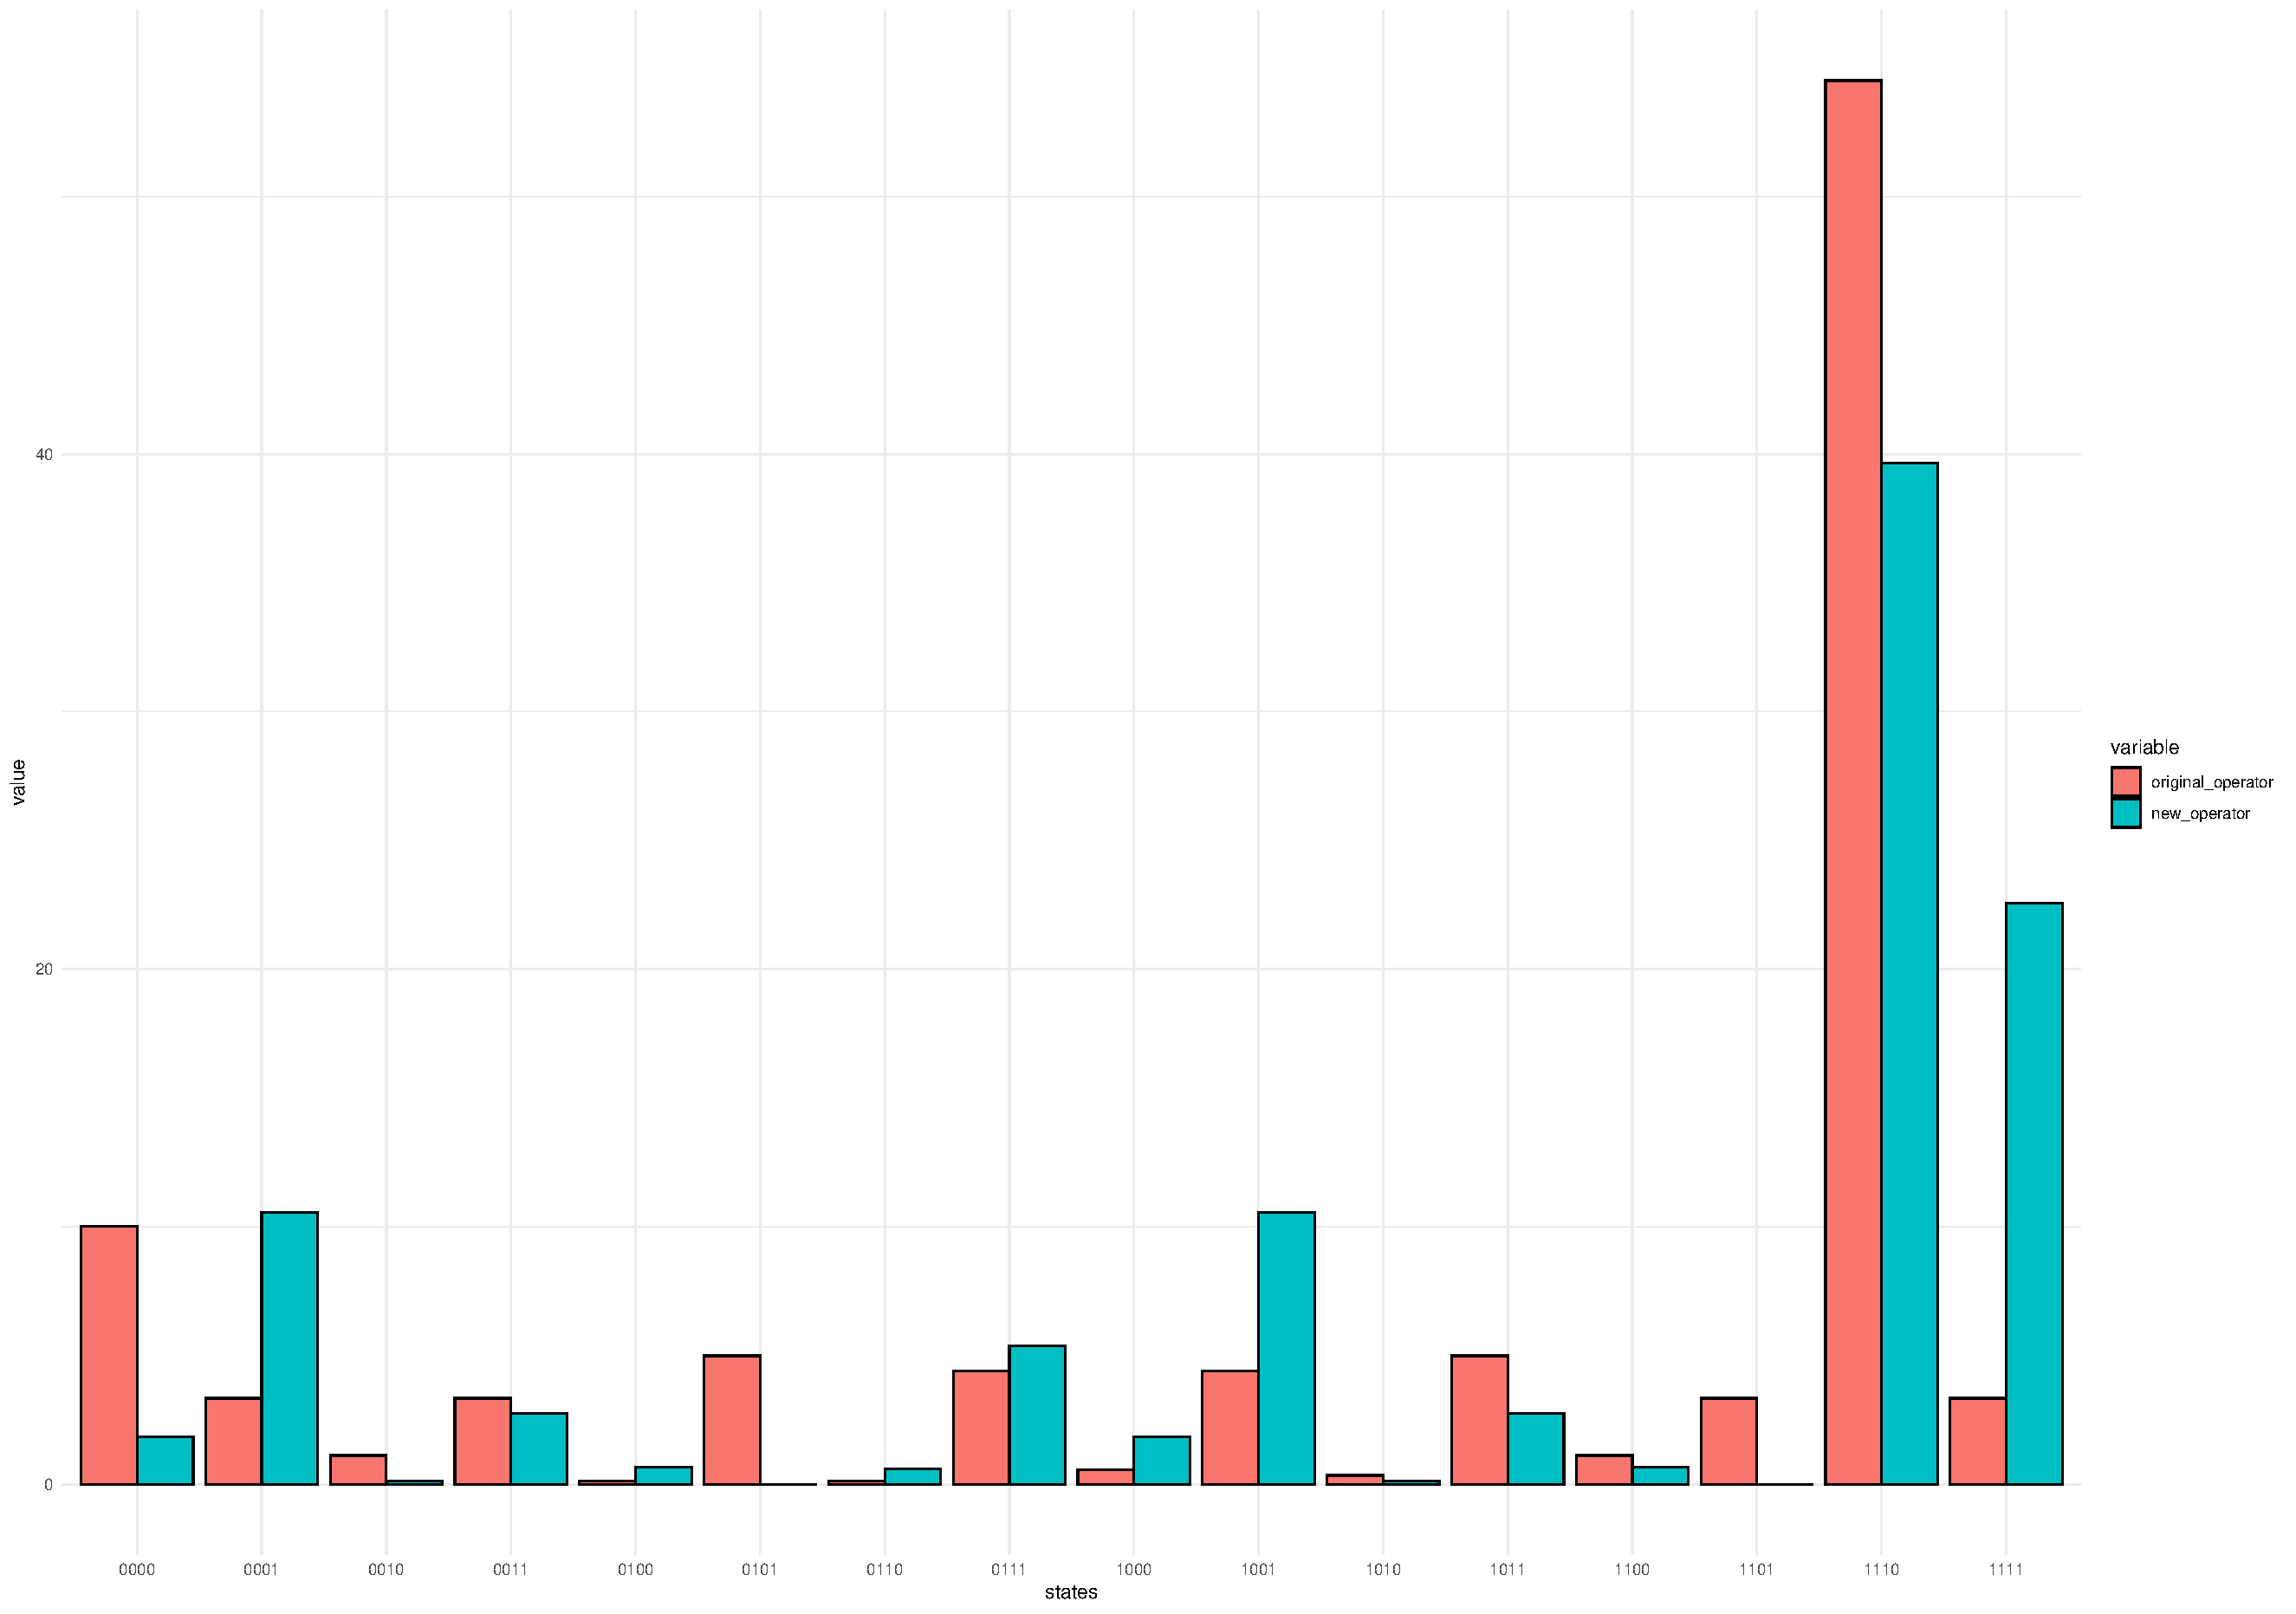
\includegraphics[width=0.9\linewidth]{figures/new_4step.pdf}
	\end{align*}
\end{frame}

\section{Conclusions and future work}
\begin{frame}{Conclusions}	
	
	The original, 'intuitive' implementation of a staggered quantum walk can be heavily optimized.
	\begin{itemize}
		\item Total number of gates
		\item T-count value
	\end{itemize}
	
	It also lead to the identification of an alternative formulation of the evolution operator.
	\begin{itemize}
		\item Significant reduction in the number of gates.
		\item Suitable for running on more limited quantum processing units.
	\end{itemize}
\end{frame}
\begin{frame}{Conclusions - (cont.)}	
	\begin{itemize}
		\item This exercise regards algorithmic optimization  in quantum programming  as a \emph{graph reconfiguration} process. 
		\item This has a huge potential in the development of hybrid quantum-classical algorithms, which are the ones that can actually run in current quantum devices.
	\end{itemize}
\end{frame}
\end{document}
